%%
%% This is file `sample-acmsmall.tex',
%% generated with the docstrip utility.
%%
%% The original source files were:
%%
%% samples.dtx  (with options: `acmsmall')
%% 
%% IMPORTANT NOTICE:
%% 
%% For the copyright see the source file.
%% 
%% Any modified versions of this file must be renamed
%% with new filenames distinct from sample-acmsmall.tex.
%% 
%% For distribution of the original source see the terms
%% for copying and modification in the file samples.dtx.
%% 
%% This generated file may be distributed as long as the
%% original source files, as listed above, are part of the
%% same distribution. (The sources need not necessarily be
%% in the same archive or directory.)
%%
%%
%% Commands for TeXCount
%TC:macro \cite [option:text,text]
%TC:macro \citep [option:text,text]
%TC:macro \citet [option:text,text]
%TC:envir table 0 1
%TC:envir table* 0 1
%TC:envir tabular [ignore] word
%TC:envir displaymath 0 word
%TC:envir math 0 word
%TC:envir comment 0 0
%%
%%
%% The first command in your LaTeX source must be the \documentclass command.
\documentclass[acmsmall]{acmart}

%%
%% \BibTeX command to typeset BibTeX logo in the docs
\AtBeginDocument{%
  \providecommand\BibTeX{{%
    \normalfont B\kern-0.5em{\scshape i\kern-0.25em b}\kern-0.8em\TeX}}}

%% Rights management information.  This information is sent to you
%% when you complete the rights form.  These commands have SAMPLE
%% values in them; it is your responsibility as an author to replace
%% the commands and values with those provided to you when you
%% complete the rights form.
\setcopyright{acmcopyright}
\copyrightyear{2018}
\acmYear{2018}
\acmDOI{XXXXXXX.XXXXXXX}

\usepackage{graphicx}
\usepackage{algorithm}
\usepackage{algpseudocode}
\newfloat{algorithm}{t}{lop}
\renewcommand{\algorithmicrequire}{\textbf{Input:}}
\renewcommand{\algorithmicensure}{\textbf{Output:}}

\newcommand{\RL}{$RL$}


%%
%% These commands are for a JOURNAL article.
\acmJournal{JACM}
\acmVolume{37}
\acmNumber{4}
\acmArticle{111}
\acmMonth{8}

%%
%% Submission ID.
%% Use this when submitting an article to a sponsored event. You'll
%% receive a unique submission ID from the organizers
%% of the event, and this ID should be used as the parameter to this command.
%%\acmSubmissionID{123-A56-BU3}

%%
%% The majority of ACM publications use numbered citations and
%% references.  The command \citestyle{authoryear} switches to the
%% "author year" style.
%%
%% If you are preparing content for an event
%% sponsored by ACM SIGGRAPH, you must use the "author year" style of
%% citations and references.
%% Uncommenting
%% the next command will enable that style.
\citestyle{acmauthoryear}

%%
%% end of the preamble, start of the body of the document source.
\begin{document}

%%
%% The "title" command has an optional parameter,
%% allowing the author to define a "short title" to be used in page headers.
\title{An Adaptive Reinforcement Learning Approach to Parameter Tuning in Genetic Algorithms}

%%
%% The "author" command and its associated commands are used to define
%% the authors and their affiliations.
%% Of note is the shared affiliation of the first two authors, and the
%% "authornote" and "authornotemark" commands
%% used to denote shared contribution to the research.

% Since it's a double-blind review, I'll use untitled author credentials here.....Marwan
\author{Author 1}
\authornote{Both authors contributed equally to this research.}
% This has been found in the template, we can alter this at any time before the submission....Marwan
\email{author1@corporation.com}
\orcid{xxxx-xxxx-xxxx}
\author{Author 2}
\authornotemark[1]
\email{author2@corporation.com}
\affiliation{%
  \institution{Institute Name}
  \streetaddress{P.O. Box xxxx}
  \city{City}
  \state{State}
  \country{Country}
  \postcode{xxxxx}
}

\author{Author 3}
\affiliation{%
  \institution{Institute Name}
%   \streetaddress{1 Th{\o}rv{\"a}ld Circle}
  \city{City}
  \country{Country}}
\email{author3@corporation.com}

\author{Author 4}
\affiliation{%
  \institution{Institute Name}
  \city{City}
  \country{Country}}
\email{author3@corporation.com}

%%
%% By default, the full list of authors will be used in the page
%% headers. Often, this list is too long, and will overlap
%% other information printed in the page headers. This command allows
%% the author to define a more concise list
%% of authors' names for this purpose.
\renewcommand{\shortauthors}{Trovato and Tobin, et al.}

%%
%% The abstract is a short summary of the work to be presented in the
%% article.
\begin{abstract}
    Genetic algorithms (GAs) are a subclass of evolutionary algorithms often used to solve difficult combinatorial or non-linear problems. However, most GAs have to be configured for a particular problem type, and even then, the performance depends on many hyperparameters and reproduction operators. 
    In this paper, a reinforcement learning (RL) approach is designed to adaptively set parameters for a GA used for solving a Capacitated Vehicle Routing Problem (CVRP). An RL agent interacts with the GA environment by taking actions that affect the parameters governing its evolution, starting from a given initial point. The results obtained by this RL-GA procedure are then compared with those obtained by alternate static parameter values. For a set of benchmark problems, the solutions obtained by the RL-GA are better (up to 11\% improvement) than those obtained for the set as compared to the alternate approach. Examination of the results shows that the RL-GA maintains great diversity in the population pool, especially as the iterations accrue. Computational runs are traced to show how the RL agent learns from population diversity and solution improvements over time, leading to near-optimal solutions.
\end{abstract}

%%
%% The code below is generated by the tool at http://dl.acm.org/ccs.cfm.
%% Please copy and paste the code instead of the example below.
%%
\begin{CCSXML}
<ccs2012>
   <concept>
       <concept_id>10003752.10010070.10010071.10010261</concept_id>
       <concept_desc>Theory of computation~Reinforcement learning</concept_desc>
       <concept_significance>500</concept_significance>
       </concept>
   <concept>
       <concept_id>10010147.10010257.10010293.10011809.10011812</concept_id>
       <concept_desc>Computing methodologies~Genetic algorithms</concept_desc>
       <concept_significance>500</concept_significance>
   </concept>
   <concept>
       <concept_id>10010405.10010481</concept_id>
       <concept_desc>Applied computing~Operations research</concept_desc>
       <concept_significance>500</concept_significance>
       </concept>
   <concept>
       <concept_id>10010147.10010169.10010170.10010174</concept_id>
       <concept_desc>Computing methodologies~Massively parallel algorithms</concept_desc>
       <concept_significance>500</concept_significance>
       </concept>
 </ccs2012>
\end{CCSXML}

\ccsdesc[500]{Theory of computation~Reinforcement learning}
\ccsdesc[500]{Computing methodologies~Genetic algorithms}
\ccsdesc[500]{Applied computing~Operations research}
\ccsdesc[500]{Computing methodologies~Massively parallel algorithms}


\keywords{Reinforcement Learning, Genetic Algorithms,Vehicle Routing Problem, Heuristics, Optimization, Tuning, Design of Experiments, Parallelism, GPU, Acceleration}


%%
%% This command processes the author and affiliation and title
%% information and builds the first part of the formatted document.
\maketitle

\section{Introduction}\label{sec:introduction}

The use of Evolutionary Algorithms (EA) for solving difficult combinatorial optimization problems is well documented in the literature \cite{ alzyadat2020genetic, baker2003genetic}. Most related heuristics or metaheuristics are tested with benchmark problems of established complexity such as the Traveling Salesman Problem (TSP) and variants, or Vehicle Routing Problems (VRPs) and variants, among others.  Genetic algorithms (GAs) are subclass of EAs that mimic a number of reproduction features to emulate natural (genetic) growth processes. These features are: chromosome selection, mating, and mutation processes \cite{bauer1994genetic}. In nature, survival of the species is assumed to be the main reward. In computational methods, a typical GA algorithm generates a population of feasible solutions (i.e., individuals or chromosomes) each of which is evaluated by a fitness function - usually related to the objective and constraints of the problem being solved. In subsequent iterations, chromosomes with the greatest fitness are selected for breeding and a crossover mechanism is applied to obtain the next generation. A mutation process is also coded to introduce diversity within the population. Iterations continue until no improvements are recorded for several generations. What distinguishes GAs from other heuristic methods is that they operate on a population of potential solutions which increases the likelihood of maintaining a good feasible solution and eventually moving to a better one. 

GAs can take many generations, and corresponding computation time, to converge. One approach to obtain good results in acceptable times is to parallelize the algorithm by either using multi-core CPU-based algorithms \cite{rey2018cpu}, or by utilizing recent hardware advances in graphics processing units (GPUs) \cite{benaini2018genetic, coelho2016integrated} that led to decreases in processing times by two to three dimensions of order \cite{abdelatti2021Op}. One of the applications involving GAs to solve combinatorial optimization problems can be found in the well-known VRP problems that gain special relevance in modern logistics and supply chain operations. VRPs involve determining optimal delivery/pick up routes for multiple vehicles through a set of locations, subject to constraints \cite{dantzig1959truck}. Many variants of the VRP have been studied: the capacitated VRP (CVRP), periodic VRP (PVRP),  VRP with time windows (VRPTW) and others. The CVRP problem is a basic form of the VRP where the total demands of the customers serviced by a vehicle cannot exceed its capacity, and the customers must be visited only once. 

GAs have been used effectively to solve many VRP scenarios \cite{baker2003genetic, garcia2009comparison}. The use of GPUs for solving VRPs has also been reported in  \cite{rey2018cpu, wodecki2015parallel}.  \cite{abdelatti2020improved} presented an improved GA incorporated with a local search algorithm for the CVRP. The proposed framework was entirely executed on a GPU and successfully provided high-quality solutions within reasonable computational times, and near-optimal solutions for smaller benchmark problems.

A common problem with GAs is the premature convergence, i.e., the inability to escape from locally optimal, but globally suboptimal, solutions. This can be addressed by preserving the population diversity, whereby a local optima can be escaped from by "jumping" to a mutant solution substantially different from the stagnant population. However, keeping the balance between speedy convergence and high diversity is not easy. The selection of appropriate parameter values for executing a GA for a particular class of problems is known as the parameter tuning problem. Correctly tuning a GA is essential for establishing a high-performing algorithm that can be used for yielding, it is a persistent challenge for developers because of the large number of options and the limited knowledge about the effect of the parameters on the performance \cite{karafotias2014parameter}.

Numerous techniques for tuning GA have been reported, including but not limited to: fuzzy logic \cite{shirazi2016fuzzy}, meta-EA \cite{grefenstette1986optimization} and design of experiments (DOE) \cite{ arin2011comparative}. \cite{bagchi1996calibration} proposed a factorial DOE-based approach for setting GA parameters considering the interaction of the crossover and mutation rates. Multiple DOE methods have been studied in \cite{arin2011comparative} for tuning GA applied to the single machine total weighted tardiness problem (TWTP). Although these methods resulted in near-optimal solutions, low efficiency remains a problem. First, solutions are obtained after many generations - this precludes their utilization as a means of finding solution for real-time systems. Second, the results obtained are sensitive to the values of several GA parameters such as mutation and crossover rates and changing these leads to instabilities of the algorithm \cite{karafotias2015evaluating}. Previous studies with self-adaptive controllers for online parameter tuning have improved solutions but suffer from premature convergence too \cite{aleti2016systematic}.

\textit{RL} is an effective learning-based controller that is used to determine parameter values for sequential stochastic decision problems. The multistage decision processes have been previously implemented in this domain for parameter selection by \cite{sakurai2010method, pettinger2002controlling, chen2005scga}. \cite{muller2002step} utilized temporal difference (TD) learning to control the mutation step size for real-valued encodings. However, these decision models have focused on utilizing an off-the-shelf evolutionary algorithm and controlling a single parameter at a time (e.g., probability of permutation) to mitigate estimating a large state-action model. These deficiencies, in turn, cause patchwork issues, which are associated with ignoring the effect of parameter interactions when solving large-scale and dynamic real-world problems.

\section{Proposed Approach}\label{sec:proposed-approach}

\begin{figure}
\begin{centering}
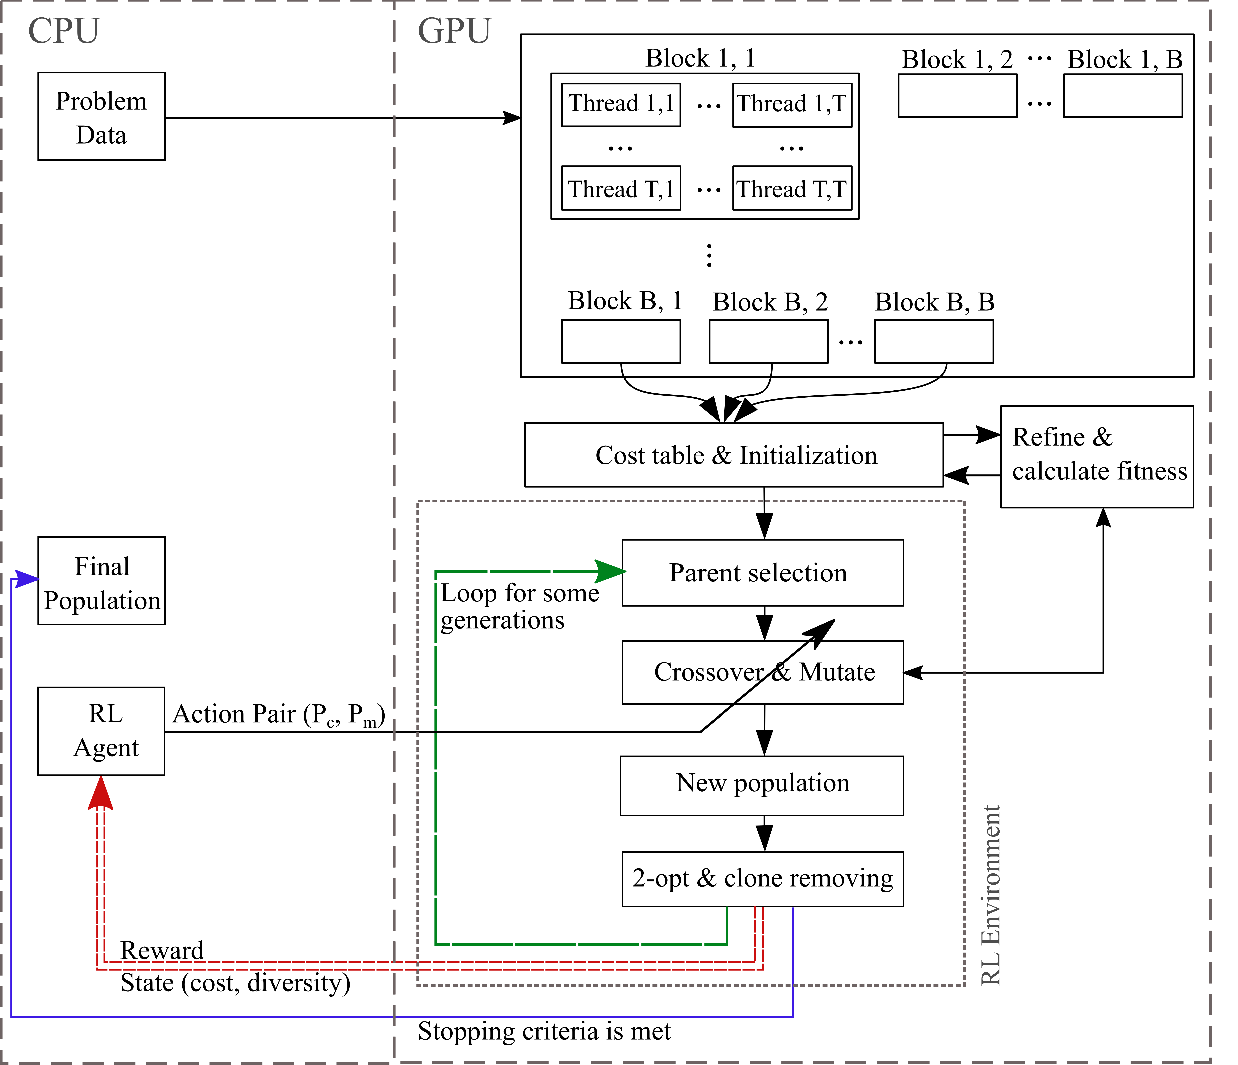
\includegraphics[scale=0.35]{figs/RL_GPU_implementation.pdf}
\par\end{centering}
\begin{centering}
\caption{Proposed RL approach for adaptive tuning of a GA\label{fig:RL-GPU}}
\par\end{centering}
\end{figure}

This paper introduces \textit{RL} as a generic control mechanism to guide the GA to decide multiple parameters, aiming to achieve near-optimal results with reduced computational cost. We tune both the mutation and crossover probabilities ($p_m$ and $p_c$ respectively) simultaneously to employ decisions based on the feedback received from the evolutionary process. More specifically, the GA environment responds to the actions taken by the \textit{RL} agent, namely the $p_m$ and $p_c$ values, and generates a new population with the associated rewards. This \textit{RL}-based parameter controller improves the performance of the algorithm towards solving large-scale and practical problems. The proposed algorithm is tested on a number of common CVRP benchmark problems in the literature.

 To evaluate the effectiveness of the proposed algorithm, we compare the results of our proposed approach with the results obtained by tuning the same GA using a design of experiments (DOE) on the same problems. The tuning settings by the DOE are the result of a two-level ($2^k$) full factorial design of experiment \cite{montgomery2017design} pilot runs on small scale problems which are then reflected on medium and large problems.

\section{RL-based parameter selection} \label{sec:\RL}
The proposed framework is defined according to the Q-learning model \cite{watkins1989learning, watkins1992q, montague1999reinforcement}, which iteratively improves the off-policy method by estimating transitions from one state-action pair to another. Therefore, to learn the value of the current policy and to improve it iteratively, we define \textit{RL} to control GA operators as follows:

\begin{itemize}
\item \textbf{State space:} The state space ($S$) is defined as a tuple of two indices, namely, the change ($C$) in the value of the best cost from the older and the recent generation, and the diversity index ($DI$) that tells the rate of the number of unique chromosomes in the new generation. It's noted from Table \ref{tab:rules} that the state space is of size $6 \times 5$ as detailed in the sequel.

\item \textbf{Action space:} The action space defined as $A$, is the tuple $(p_{m}, p_{c})$, where $p_m$ and $p_{c}$ denote the mutation and the crossover rate respectively. The ranges of each of these two parameters are from $0$ to $1$ discretized separately into $d=10$ intervals, and therefore, create $d^2=100$ possible action pairs.

\item \textbf{Estimated state-action:} Q-learning is a values-based learning algorithm, which updates the value function ($Q$) for each state-action pair ($(S,A)$) in Q-table using the following Bellman equation:

\begin{equation}\label{eq:Qfun}
\begin{aligned}
    Q(S(t), A(t)) \leftarrow (1-\alpha)Q(S(t), A(t)) + \\
    \alpha(R(t)+\gamma \max\limits_{A(t+1)} Q(S(t+1), A(t+1)))
\end{aligned}    
\end{equation}

The selection of an action is made based on the epsilon-greedy policy, and this policy chooses a random action either from the Q-table with a probability $\epsilon$, or picks the greedy action with the highest Q-value. 
% \newline
\item \textbf{Reward:} The reward $R$ is determined based on the state $S$ returned from the GA environment using two indices: the cost improvement $C$ and the diversity index $DI$. Table \ref{tab:rules} shows the returned reward values based on different $C$ and $DI$ levels. The rows in the table correspond to the possible values of the cost improvement ($C$); from very high change (VHC) to very low change (VLC) as well as a stalled state and an increase in cost; whereas the columns correspond to five possible values for the diversity index ($DI$) from very high diverse (VHD) to very low diverse (VLD).
\end{itemize}

\begin{table}[h]
\begin{tabular}{c|ccccc}
\toprule
          & VHD   & HD    & MD    & LD    & VLD   \\
\midrule
VHC       & 200   & 150   & 100   & 50    & 25    \\
HC        & 150   & 112.5 & 75    & 37.5  & 18.75 \\
LC        & 100   & 75    & 50    & 25    & 12.5  \\
VLC       & 50    & 37.5  & 25    & 12.5  & 6.25  \\
Stalled   & 0     & 0     & -10   & -20   & -30   \\
Increased & -1000 & -1500 & -2000 & -2500 & -3000 \\
\bottomrule
\end{tabular}
\caption{Rule table for reward values \label{tab:rules}}
\end{table}


\begin{algorithm}[h]
    \caption{\textit{RL}-enabled GA for tuning the hyperparameters}
    \label{alg:\RL-GA}
    
    \begin{algorithmic}[h]
    \Require Population $(Population)$: initial population at t=0  \\ $\quad \;$ 
    States $(S)$: $\{C, DI\}$    \\ $\quad \;$
    Action $(A)$: $\{(p_{c0}, p_{m0}), (p_{c0}, p_{m1}), \dots, (p_{c99}, p_{99})\}$ \\ $\quad \;$
    % Action $(A)$: $\{(+p_{c}, +p_{m}), (-p_{c}, -p_{m}), $      \\ $\quad \quad \quad \quad \quad \quad \; \;\;  \; \;$ 
    %               $(+p_{c}, -p_{m}), (-p_{c}, +p_{m}), \text{No change}\}$   \\ $\quad \;$ 
    Reward function $(R)$: $S \times A \rightarrow \, \mathbb{R}$ \\ $\quad \;$ 
    Probabilistic transition function $(Transition)$: $ S \times A \rightarrow S $  \\ $\quad \;$ 
     Parameters: $\{\delta, \lambda, \gamma, \epsilon, \alpha \} $               
%   \\
        \Function{GA\RL} {$.$} 
             \State $Q (S(t), A(t)) \leftarrow \text{initialize} $
                \While {$Q(S(t),A(t))$ is not converged}
                \State {Use State Set $S(t)$}
                    \While {$t<T$}
                \State {$p_{c} \leftarrow S(t).SetCrossoverProb()$}
                \State {$p_{m} \leftarrow S(t).SetMutationProb()$}
                \State {$Population(t) \leftarrow Population(t).SelectedGenes$}
                \State {$Population(t) \leftarrow Population(t).\text{GA}(p_{c}, p_{m})$}
                
                \State {$R(t) \leftarrow Population(t).Reward()$}
                 
                \State {$S(t+1) \leftarrow  S(t).Transition(A(t))$}
                \State {$A(t) \leftarrow S(t).\pi(A(t))$}
               
                
                \State {$Q(S(t+1),A(t)) \leftarrow (1-\alpha)Q(S(t),A(t))+\alpha(R(t)$}
                % \State {$Population(t+1) \leftarrow Population(t).SelectedGenes$}
                % \State {$Population(t+1) \leftarrow Population(t).\text{GA}(p_{c}, p_{m})$}
                
                % \State {$R(t) \leftarrow Population(t+1).Reward()$}
                 
                % \State {$S(t+1) \leftarrow  S(t).Transition(A(t))$}
                % \State {$A(t+1) \leftarrow S(t).\pi(A(t))$}
               
                
                % \State {$Q(S(t+1),A(t)) \leftarrow (1-\alpha)Q(S(t),A(t))+\alpha(R(t)$}
                \State \quad \quad \quad \quad \quad \quad \quad  {$+ \gamma \max\limits_{A(t+1)} Q(S(t+1),A(t+1)))$}
                % \State \quad \quad \quad \quad \quad \quad \quad \quad  {$+ \gamma \max\limits_{A(t+1)} Q(S(t+1),A(t+1)))$}
                \State {$Population(t) \leftarrow Population(t+1)$}
                \State {$S(t) \leftarrow S(t+1)$}
                \State $t \leftarrow t+1$
                    \EndWhile
                    
                \EndWhile
                \EndFunction
            \Ensure {$Population(t=T), R(t=T)$}
    \end{algorithmic}
\end{algorithm}

As opposed to the conventional GA, where the mutation and crossover rates $p_m$ and $p_c$ are fixed throughout the run, our approach depicted in Figure \ref{fig:RL-GPU} involves an adaptive change of these parameters. The population during the current state is denoted as Population($t$), and its evolution to Population($t+1$) is governed by the values of $p_c$ and $p_m$ for the current state. The GA applies the selected values for parameters only for a fixed number of generations after which the reward is returned to the \textit{RL} agent. The expected long-term impact and the influence of the action from this state are updated based on the reward value $R$. As a result, the proposed framework preserves the best chromosomes and changes the parameter values as the algorithm iterates. The learning rate ($\alpha$) is used to control the influence of the target on the current Q-values. Since the target is the TD between two updates by the \textit{RL}, it will be influenced by the improvement scale problem of GA. As the GA evolves, improvements to the fitness value will taper off. Consequently, we only consider the fitness value of the current generation. When GA is evolving, the learning rate of \textit{RL} is controlled to decrease the influence of the target on the learned Q-values to prevent fitness decay. A complete pseudocode algorithm for the \textit{RL} part of RL-GA is given in Algorithm \ref{alg:\RL-GA}. Interested readers can clone the functioning code from the GitHub repository\footnote{https://github.com/J-Que/RL-GA}.

\section{Computational Results}\label{sec:exectution-results}
To test the performance of the RL-GA, several instances of benchmark problems from the literature were solved, and the results are reported in~Table \ref{tab:results}. Problems involving $40$ to $70$ customer nodes were selected, as well as a larger 200 node problem. Each problem was solved five times using the RL-GA algorithm. The first column on Table~\ref{tab:results} is the sequence number. Column 2 is the problem label and it details the number of nodes and the number of vehicles. Column 3 is the best known solution as reported by the site\footnote{http://vrp.atd-lab.inf.puc-rio.br/index.php/en/}.  Column 4 is the best solution obtained by the GA algorithm run only on a CPU. Column 5 reports the results obtained by solving the problem using a GPU version of the algorithm, as detailed in \cite{abdelatti2020improved}. $p_m$ and $p_c$ for the results in Columns 4 and 5 were set based on a Design of Experiments approach, detailed in \cite{abdelatti2021Op}. The sixth column reports the results of the RL-GA algorithm and the last two columns report the average value of the results  obtained from the five runs and their respective standard deviation.


\begin{table*}
% \scalebox{.75}{
\begin{tabular}{cccccccc}
\toprule
   & Problem   & \begin{tabular}[c]{@{}c@{}}Published\\    Optimal\end{tabular} & GPU-GA & CPU-GA & RL-GA    & \begin{tabular}[c]{@{}c@{}}Average\\    RL-GA\end{tabular} &  \begin{tabular}[c]{@{}c@{}}Std Dev\\    RL-GA\end{tabular}\\
\midrule
1   & B-n31-k5    & 672           & 691   & 677   & 672*  & 675.6   & 4.41   \\
2   & B-n45-k5    & 751           & 840   & 762   & 751*  & 756     & 4.29   \\
3   & B-n50-k8    & 1312          & 1329  & 1327  & 1316  & 1324    & 4.15   \\
4   & M-n200-k17  & 1373          & 1473  & 1598  & 1434  & 1482.6  & 34.3   \\
5   & P-n16-k8    & 450           & 450   & 450   & 450*  & 450     & 0      \\
6   & P-n20-k2    & 216           & 216   & 216   & 216   & 216     & 0      \\
7   & P-n21-k2    & 211           & 211   & 211   & 211   & 211     & 0      \\
8   & P-n22-k8    & 603  & 590   & 592   & 590*  & 596.2   & 5.04   \\
9   & P-n23-k8    & 529           & 529   & 529   & 529*  & 529     & 0      \\
10  & P-n40-k5    & 458           & 479   & 478   & 458*  & 465.2   & 9.37   \\
11  & P-n55-k15   & 989 & 1058  & 975*  & 981   & 996     & 9.93   \\
12  & P-n70-k10   & 827           & 845   & 892   & 853   & 865.2   & 11.29  \\
\bottomrule
\end{tabular}
% }
\begin{centering}
\caption{Runs results and comparisons \label{tab:results}}
\par\end{centering}
\end{table*}

As can be seen from Table~\ref{tab:results}, RL-GA shows equal or better performances than the CPU-GA and the GPU-GA implementations for eleven of the twelve problems. For problem 8 (P-n22-k8), all the GA implementations improve the best known solution, and for problem 11 (P-n55-k15), the CPU-GA finds a better solution than the current best known solution. The averaged results also demonstrate equal or better performance than the GPU-GA for nine of the twelve problems, showing its consistency.

\begin{figure}[t] 
\begin{centering}
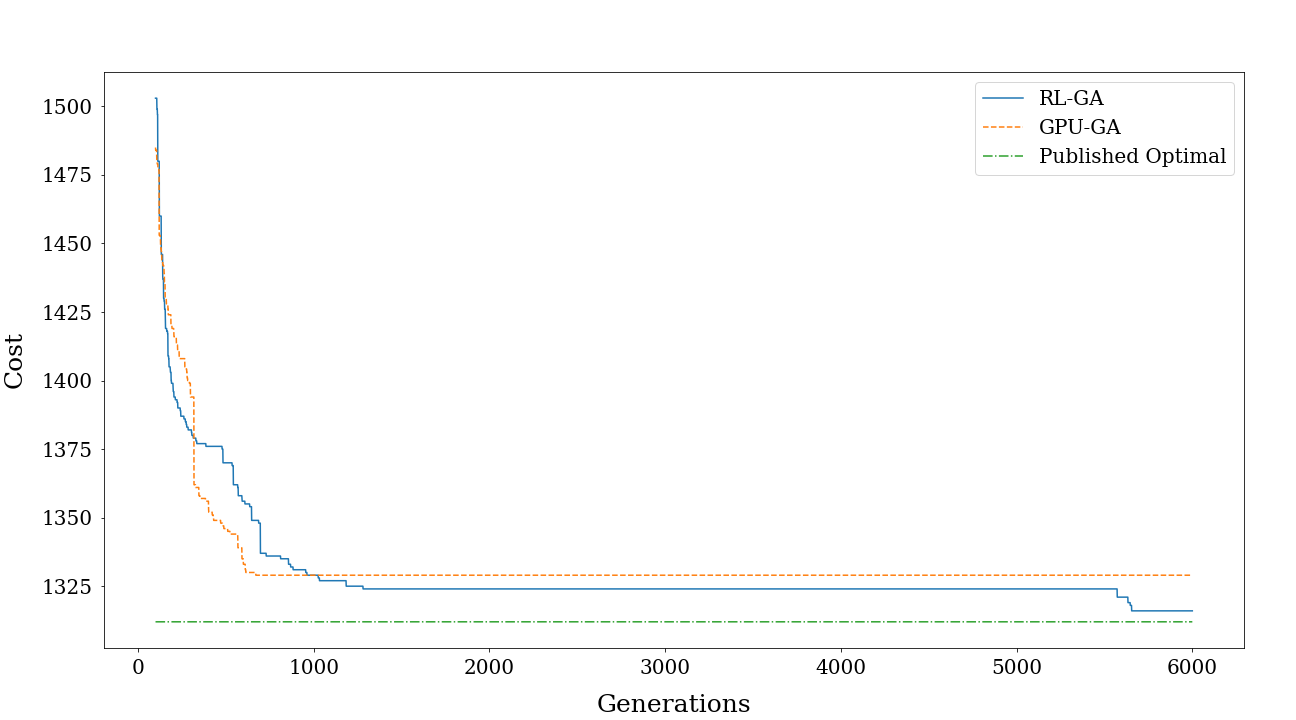
\includegraphics[scale=0.17 , trim={0 0 0 70},clip]{figs/Cost vs Generations 50 nodes.png}
\par\end{centering}
\begin{centering}
\caption{Solution trajectory for B-n50-k8}\label{fig:solnbn50}
\par\end{centering}
\end{figure}

Figure~\ref{fig:solnbn50} illustrates example trajectory (i.e., cost vs generations) taken whilst solving problem 3 (B-n50-k8). Here it can be seen that RL-GA finds a better solution than the DOE tuned GA. This also manifests when examining the solutions of the other problems tested, except for problem 12 where the GPU-GA ultimately attains a better solution.

\begin{figure}[h] 
\begin{centering}
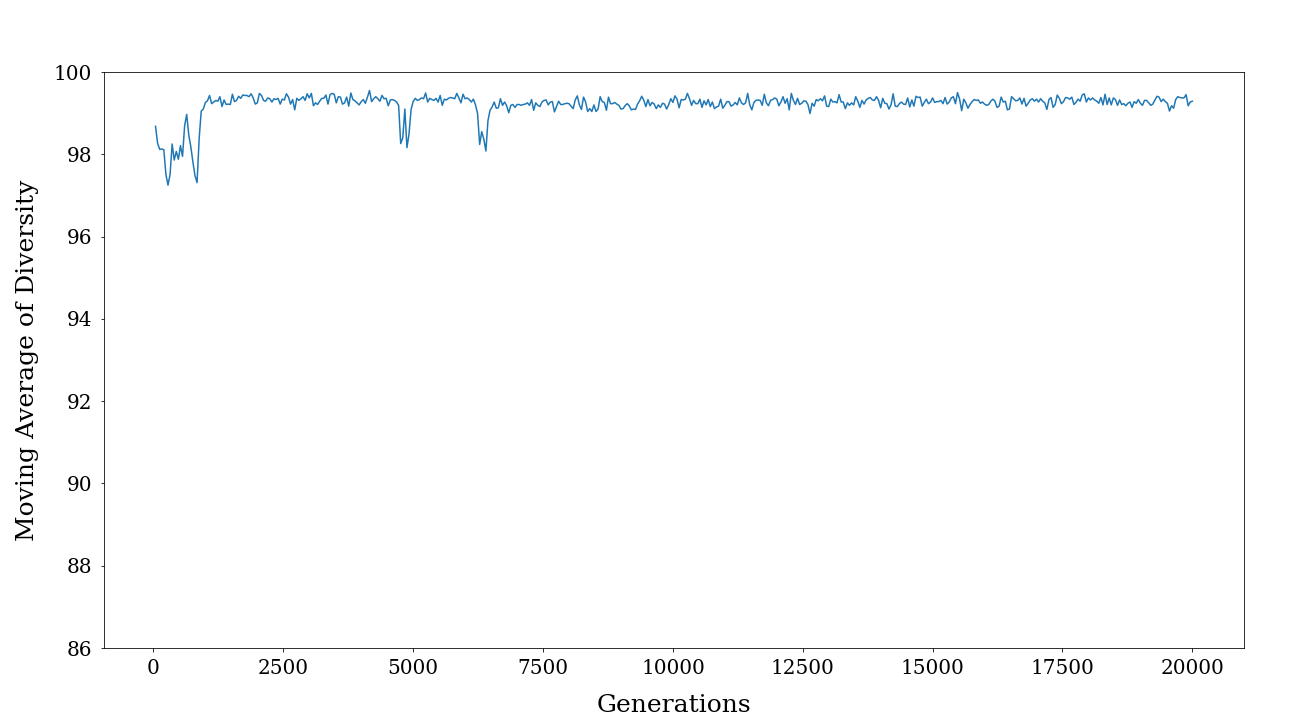
\includegraphics[scale=0.17]{figs/moving average diversity GPU-GA2.png}
\par\end{centering}
\begin{centering}
\caption{Solution diversity for B-n50-k8 with GPU-GA }\label{fig:diversityGPUGA50}
\par\end{centering}
\end{figure}


\begin{figure}[h] 
\begin{centering}
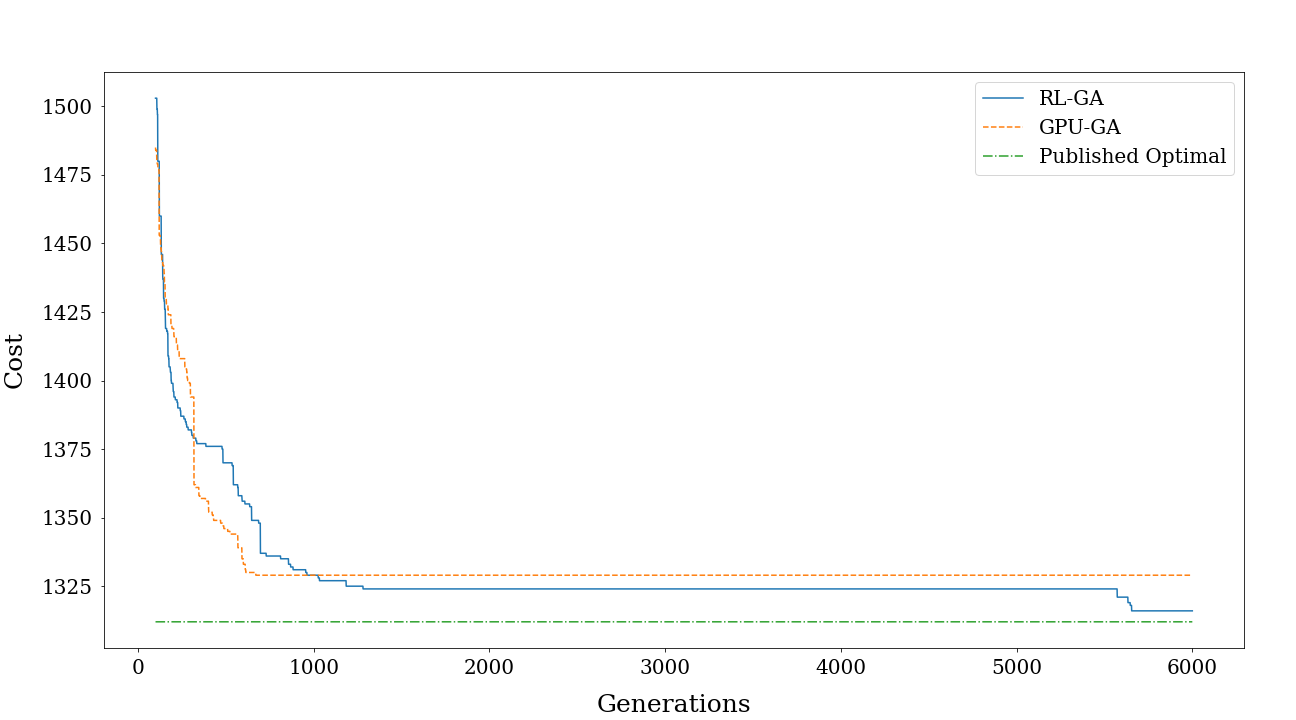
\includegraphics[scale=0.17]{figs/moving average diversity RL-GA.png}
\par\end{centering}
\begin{centering}
\caption{Solution diversity for B-n50-k8 with RL-GA}\label{fig:diversityRLGA50}
\par\end{centering}
\end{figure}

Figures %s~\ref{fig:diversityGPUGA50} and 
\ref{fig:diversityGPUGA50} and \ref{fig:diversityRLGA50} show the diversity changes over the course of the entire run for problem (B-n50-k8). From the figures, it can be observed that RL-GA biases against population diversity when the objective solutions are improving rapidly, and towards increasing diversity when the solution stagnates. % Furthermore, the RL-GA retains a greater diversity (higher overall value) throughout the run. 
This is indeed the behavior that we wanted to inculcate - and is evidence that the reward function is therefore correctly defined. 


\section{Conclusions}\label{sec:conclusions}
In this paper, a reinforcement learning (RL) approach has been designed to adaptively set parameters for a genetic algorithm (GA) used to solving a Capacitated Vehicle Routing Problem (CVRP). For a set of benchmark problems, the solutions obtained by the RL-GA are better than those obtained for the same set of problems using a static, Design of Experiments-based approach. The RL-GA appears to be promising in that it is able to maintain greater diversity in the population pool.  Tests with problems involving a greater number of nodes for the CVRP are  planned and these will require significant computing effort. Successful with  larger problem sets, will add to the methods that can be used to obtain good solutions for complex practical problems using genetic methods with reasonable computing effort.
Since the approach presented here acts on parameters that are fundamental to all genetic algorithms, they can widely be implemented for solving other combinatorial and nonlinear optimization problems utilizing GAs.   

\bibliographystyle{ACM-Reference-Format}
\bibliography{acmart}

\end{document}
\endinput
%%
%% End of file `sample-acmsmall.tex'.
